
\documentclass[border=10pt]{standalone}
\usepackage{pgfplots}
\usepackage{amsmath}
\pgfplotsset{compat=1.18}
\begin{document}
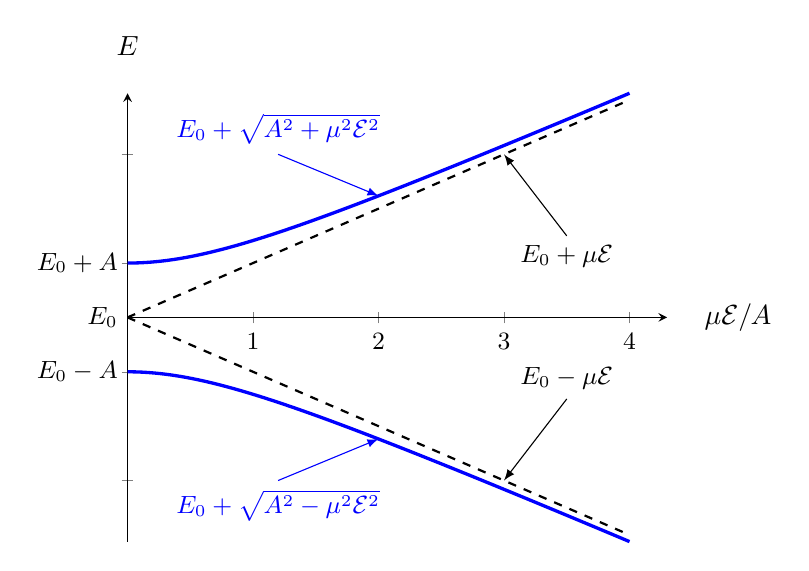
\begin{tikzpicture}
    \def\E0{1.0}
    \def\A{1.0}
    \def\m{1.84}
    \begin{scope}
        \begin{axis}
        [
            %axis line style={shorten >=-10pt, shorten <=-10pt},
            axis y line = center,
            axis x line = middle,
            axis x line shift= -\E0,
            no markers,
            xmin = 0,
            xmax = 4.3,
            clip = false,
            %enlargelimits = false,
            % ytick={1.6 ,1.85},
            yticklabels=\empty,
            xtick={1, 2, 3, 4},
            % xticklabels={, , , $\omega_0$, , ,},
            xlabel style={
                        anchor=west,
                        at={(ticklabel* cs:1.0)},
                        xshift=10pt
            },
                    ylabel style={
                        anchor=south,
                        at={(ticklabel* cs:1.0)},
                        yshift=10pt
                    },
            xlabel=$\mu\mathcal{E}/A$,
            ylabel=$E$,
            every x tick label/.append style={font=\small} 
        ]
        \addplot+[blue, very thick, domain=0:4, samples=250] {\E0 + \A*sqrt(1 +  \x*\x)};
        \addplot+[blue, very thick, domain=0:4, samples=250] {\E0 - \A*sqrt(1 +  \x*\x)};
        \draw[dashed, thick] (axis cs:0, \E0) -- (axis cs:4, \E0 + 4*\A);
        \draw[dashed, thick] (axis cs:0, \E0) -- (axis cs:4, \E0 - 4*\A);
        \node[left, font=\small] at (axis cs:0, \E0) {$E_0 $};
        \node[left, font=\small] at (axis cs:0, \E0+\A) {$E_0 + A$};
        \node[left, font=\small] at (axis cs:0, \E0-\A) {$E_0 - A$};
        \node[above, font = \small, blue] at (axis cs: 1.2, \E0+3) {$E_0 + \sqrt{A^2+\mu^2 \mathcal{E}^2}$};
        \draw[-latex, blue]  (axis cs: 1.2, \E0+3) to (axis cs: 2, {\E0 + \A*sqrt(5)});
        \node[below, font = \small, blue] at (axis cs: 1.2, \E0-3) {$E_0 + \sqrt{A^2-\mu^2 \mathcal{E}^2}$};
        \draw[-latex, blue]  (axis cs: 1.2, \E0-3) to (axis cs: 2, {\E0 - \A*sqrt(5)});

        \node[below, font = \small] at (axis cs: 3.5,\E0+1.5) {$E_0 +\mu \mathcal{E}$};
        \node[above, font = \small] at (axis cs: 3.5,\E0-1.5) {$E_0 -\mu \mathcal{E}$};
        \draw[-latex] (axis cs: 3.5,\E0+1.5) to (axis cs:3, {\E0 + 3*\A});
        \draw[-latex] (axis cs: 3.5,\E0-1.5) to (axis cs:3, \E0 - 3*\A);

        
        \end{axis}
    \end{scope}
    
\end{tikzpicture}
\end{document}